\documentclass[aspectratio=169]{beamer}

% Document metadata
\title{\vspace{0.5cm}\Large Optimal Design of Agile Jumping Maneuvers for a Single Leg System}
\subtitle{\small  Andrea Patrizi, Francesco Ruscelli, Arturo Laurenzi and Nikos G. Tsagarakis \vspace{1cm}}
\institute{Istituto Italiano di Tecnologia}

% Image for the title page (use includegraphics option to properly size/place it)
\titlegraphic{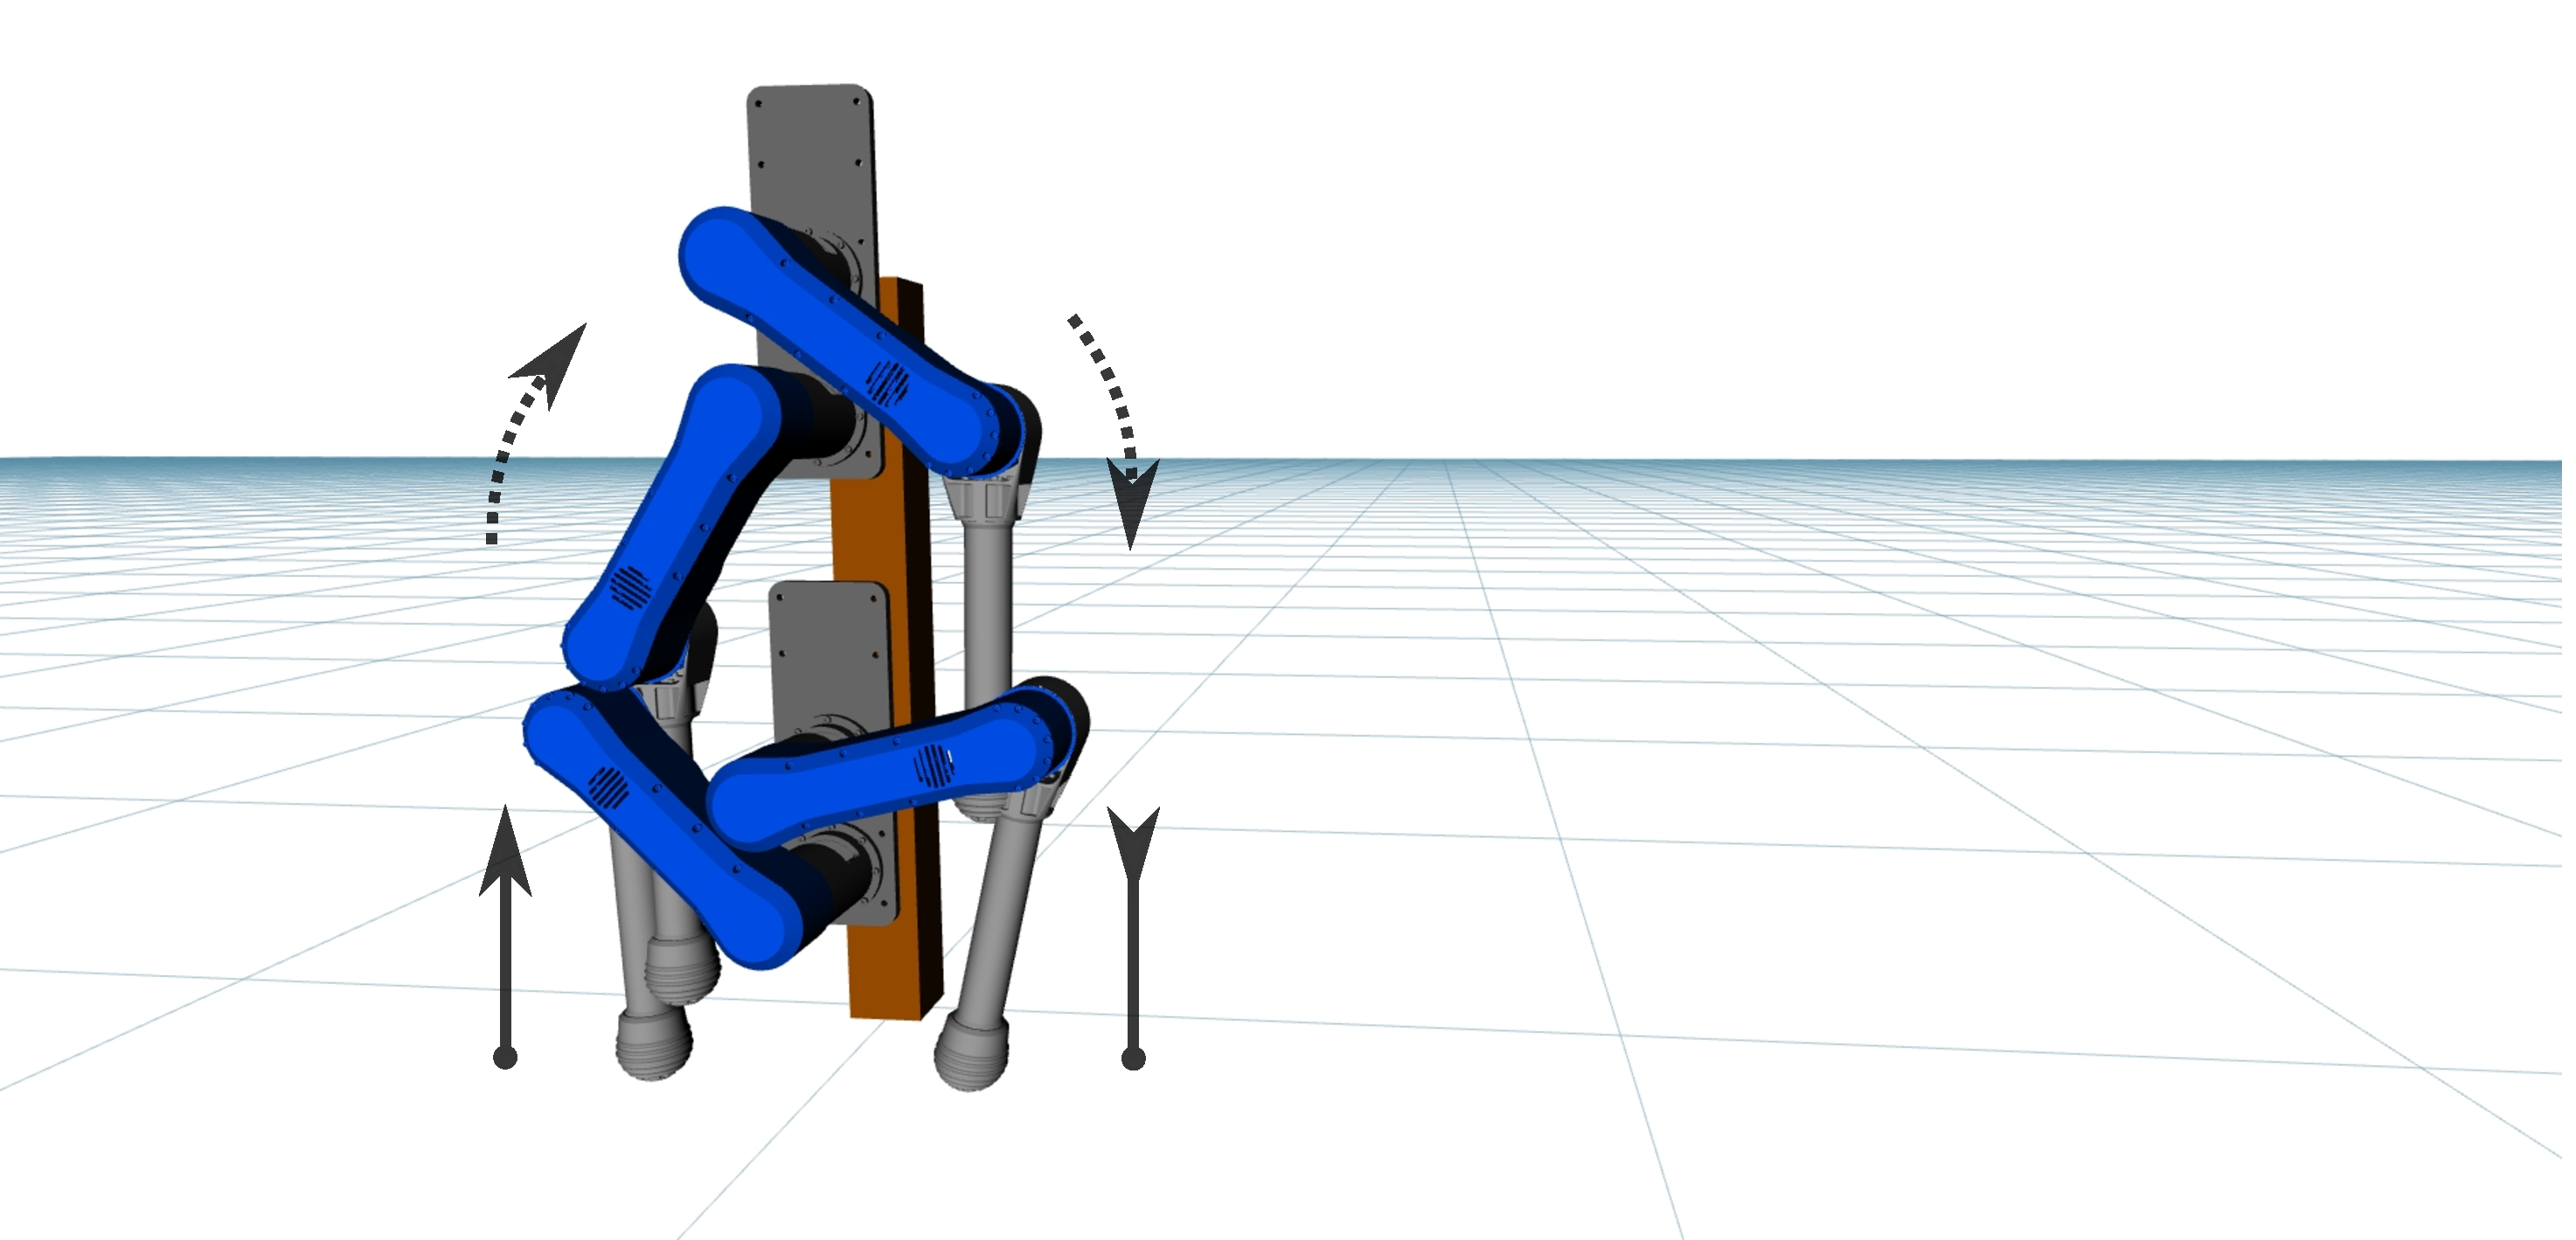
\includegraphics[width = 0.88\paperwidth]{beamer_imgs/front_slide.pdf}}

\usetheme[sectionstyle=style2]{trigon}

% Define logos to use (comment if no logo)
\biglogo{logos_and_co/iit-hhcm-logo-2} % Used on titlepage only
\smalllogo[scale = 0.25]{logos_and_co/iit-hhcm-logo-2} % Used on top right corner of regular frames

\usepackage{appendixnumberbeamer} % To use \appendix command
\pdfstringdefDisableCommands{% Fix hyperref translate warning with \appendix
  \def\translate#1{#1}%
}
\usepackage{caption} % For subfigures
\usepackage{subcaption} % For subfigures
\usepackage{xspace}
\newcommand{\themename}{\textbf{\textsc{trigon}}\xspace}

\usepackage{booktabs} % Better tables

\newcommand{\quotes}[1]{``#1''}

\usepackage{algorithm}
\usepackage{algpseudocode}
\renewcommand{\algorithmiccomment}[1]{\hspace{2em}// #1}

\usepackage{multicol}

\usepackage{hyperref}

\begin{document}

\titleframe

%\begin{frame}
%\frametitle{\Large Motivations and context}
%Driving challenge:
%\begin{itemize}
%\item Development of control and hardware for new \textbf{heavy-duty} and \textbf{agile} \textbf{electrically-powered} quadruped.
%\end{itemize}
%\end{frame}

%%%%%%%%%%%%%%%%%%%%%%%%%%%%%%%%%%%%%%%%%%%%%%%%%%%%%%%%%%%%%%%%%%

\begin{frame}
\begin{multicols}{2}
\vfill\null
Experimental setup: 
\begin{itemize}
\item 2 d.o.f \textbf{electrically-powered}, \textbf{torque-controllable} quadruped leg prototype, $50:1$ gear ratio
\item 1 d.o.f. sliding guide
\item $25\,\mathrm{Ah}$, $51.2\,\mathrm{V}$ \textbf{battery} unit, $100\,\mathrm{A}$ peak discharge current
\item dedicated \textbf{power sensing setup} for measuring regenerative power
\end{itemize}
\vfill\null
\columnbreak
\vfill\null
\vspace{0.5cm}
\begin{figure}
    \centering
    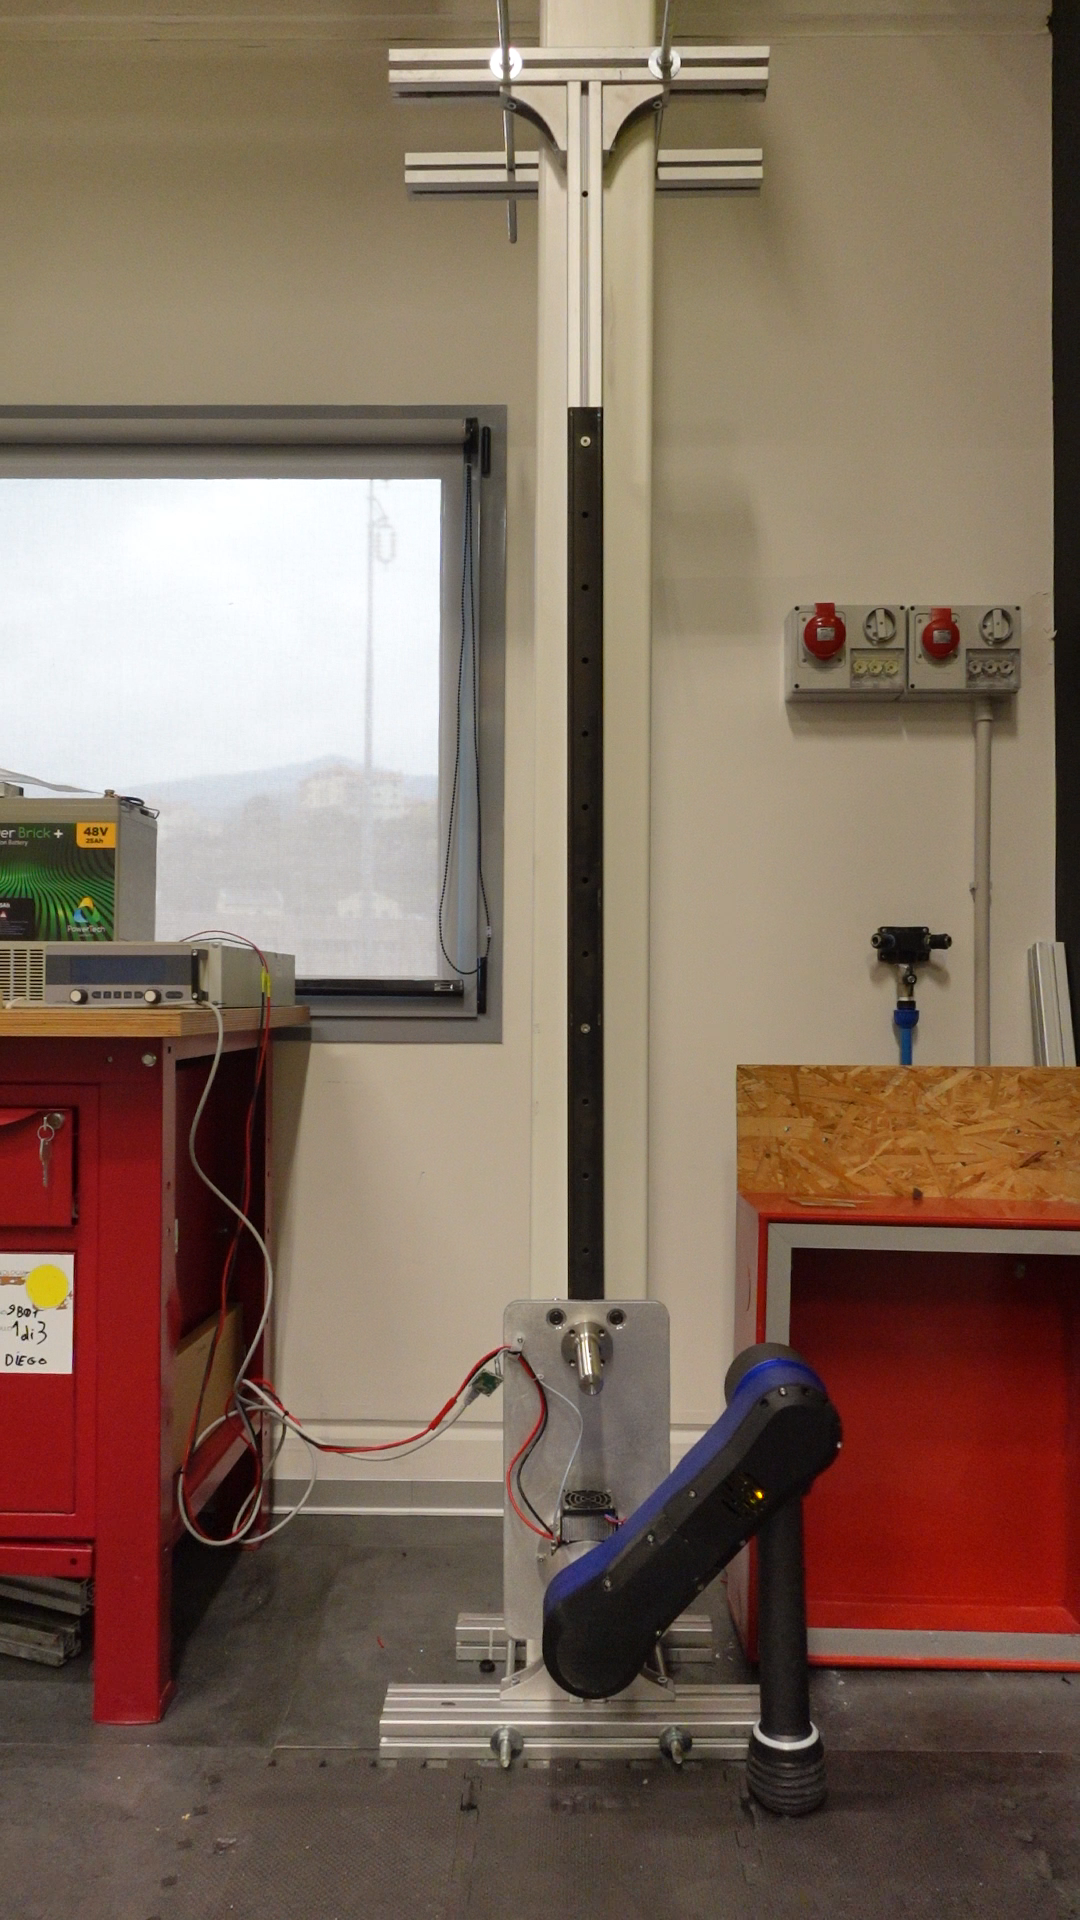
\includegraphics[width=0.5\columnwidth]{beamer_imgs/jump_sequence_intro_image/real1.png}
\end{figure}
\end{multicols}
\end{frame}

%%%%%%%%%%%%%%%%%%%%%%%%%%%%%%%%%%%%%%%%%%%%%%%%%%%%%%%%%%%%%%%%%%

%\begin{frame}
%Given the scope of our project and our experimental setup, we showcase a study revolving around
%\begin{itemize}
%\item The \textbf{design} and execution of \textbf{agile jumping maneuvers} 
%\end{itemize}
%\end{frame}

%%%%%%%%%%%%%%%%%%%%%%%%%%%%%%%%%%%%%%%%%%%%%%%%%%%%%%%%%%%%%%%%%%
%
%\begin{frame}
%\frametitle{\Large Contributions}
%We expand upon
%\begin{itemize}
%\item \textbf{Challenges} and peculiarities of the \textbf{jumping task}
%\end{itemize}
%exploiting
%\begin{itemize}
%\item \textbf{Trajectory Optimization} (TO) as our main investigation tool
%\end{itemize}
%\end{frame}

%%%%%%%%%%%%%%%%%%%%%%%%%%%%%%%%%%%%%%%%%%%%%%%%%%%%%%%%%%%%%%%%%%

\begin{frame}
\begin{multicols}{2}
\vfill\null
Jump decomposed into
\begin{itemize}
\item Take-off + flight
\item Impact + braking
\end{itemize}
\vfill\null
\columnbreak
\vfill\null
\begin{figure}
    \centering
    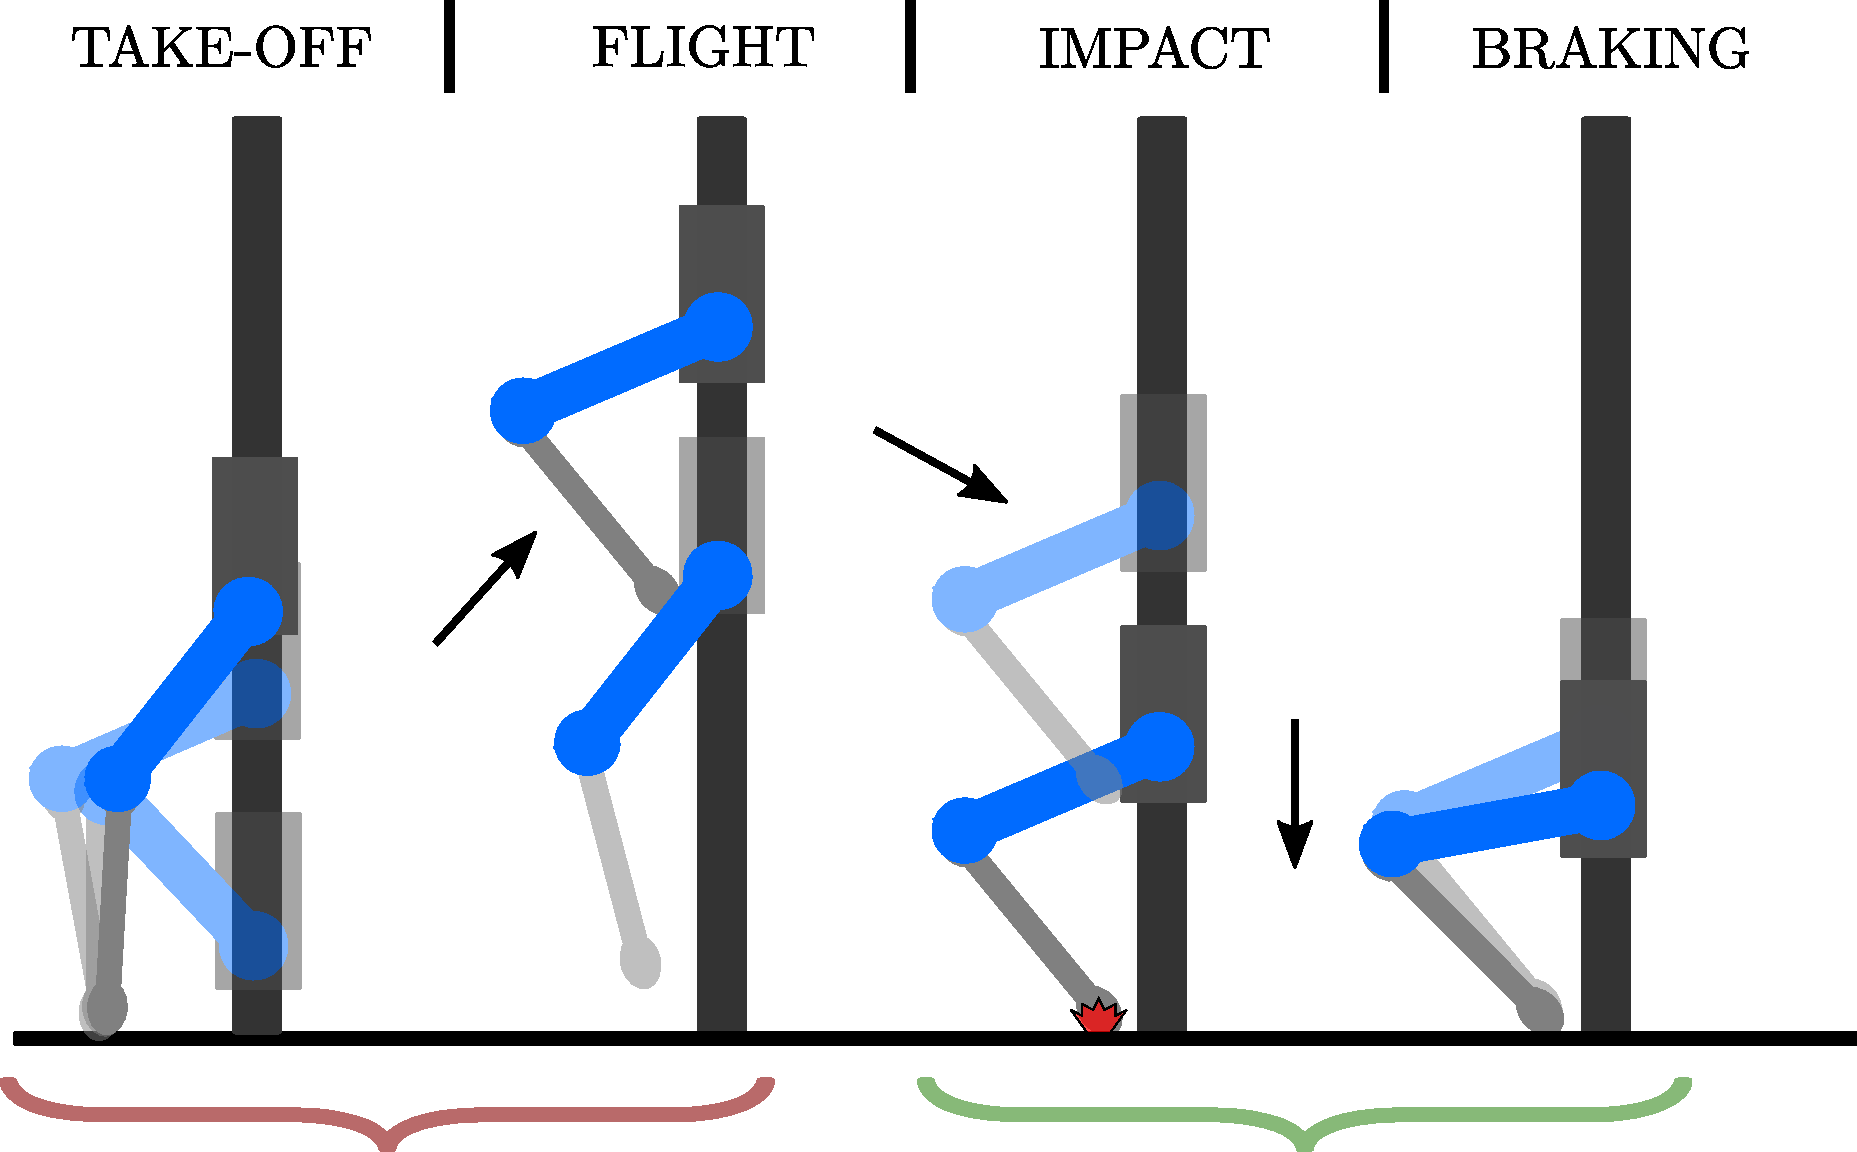
\includegraphics[width=1.0\columnwidth]{beamer_imgs/impact_opt_intro/jump_phases.pdf}
\end{figure}
\end{multicols}
\end{frame}

%%%%%%%%%%%%%%%%%%%%%%%%%%%%%%%%%%%%%%%%%%%%%%%%%%%%%%%%%%%%%%%%%%

%
%\begin{frame}
%And develop a
%\begin{itemize}
%\item \textbf{Two-stage pipeline} for the design and execution of jumping maneuvers
%\end{itemize}
%made of two coupled offline TOs.
%\vfill
%\end{frame}

%%%%%%%%%%%%%%%%%%%%%%%%%%%%%%%%%%%%%%%%%%%%%%%%%%%%%%%%%%%%%%%%%%

\begin{frame}
\frametitle{\Large}
\begin{multicols}{2}
\vfill\null
\begin{figure}
    \centering
    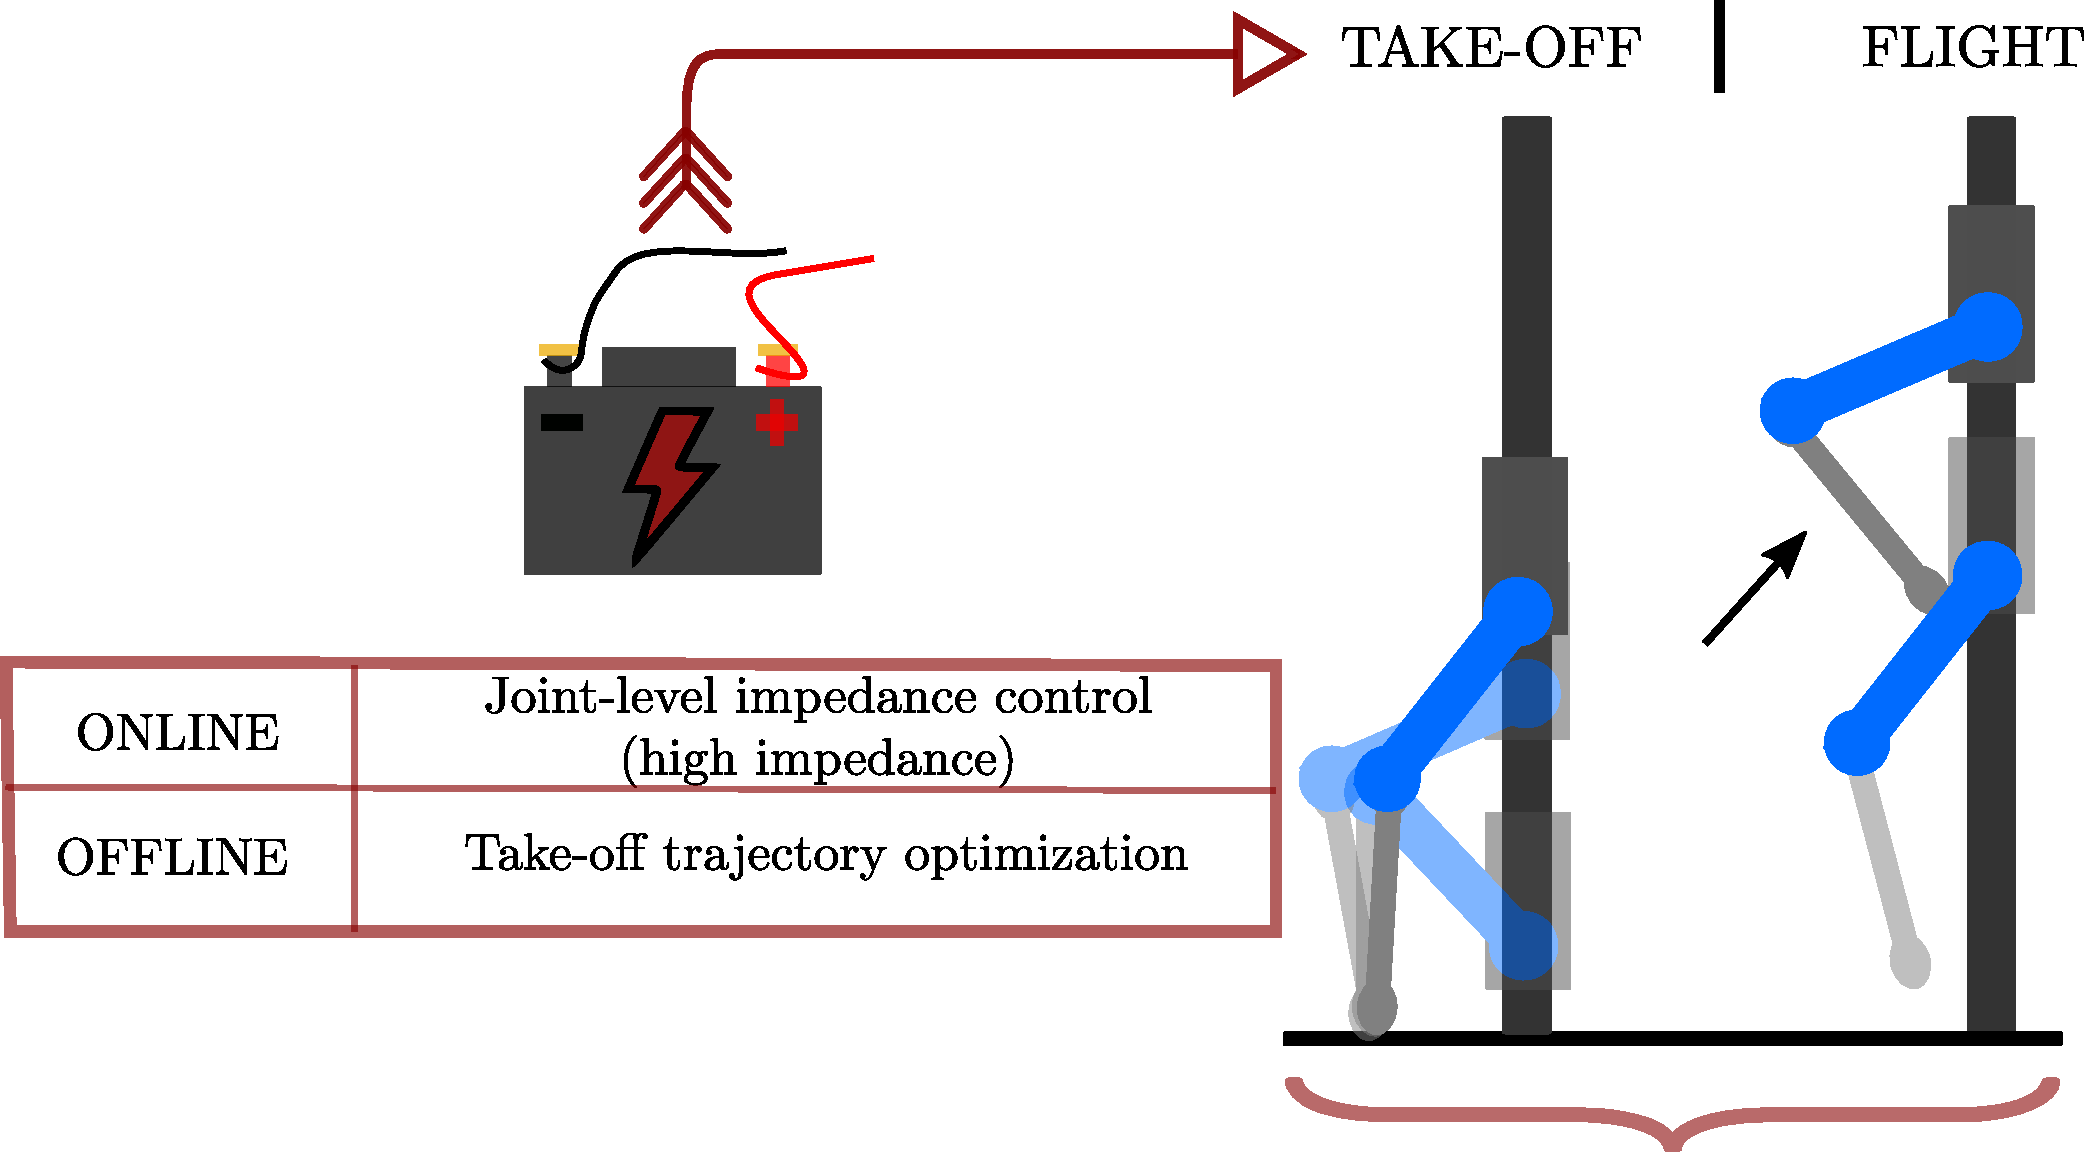
\includegraphics[width=1.0\columnwidth]{beamer_imgs/impact_opt_intro/first_TO.pdf}
\end{figure}
\columnbreak
Optimal \textbf{thrust trajectory} (first TO):
\begin{itemize}
\item {Maximizing \textbf{apex height}}\vspace{0.2cm}
\item {Minimizing \textbf{optimization-to-reality gap}:}
\begin{itemize}\vspace{0.2cm}
\item {Accurate \textbf{actuation model}s}
\item {Solution \textbf{refinement} + jerk-yank \textbf{regularization}}
\end{itemize}
\end{itemize}
\vfill\null
\end{multicols}
\end{frame}

%%%%%%%%%%%%%%%%%%%%%%%%%%%%%%%%%%%%%%%%%%%%%%%%%%%%%%%%%%%%%%%%%%

\begin{frame}
\frametitle{\Large}
\begin{multicols}{2}
Optimal \textbf{landing configuration} + braking \textbf{joint impedance} setpoints (second TO):
\begin{itemize}
\item Minimizing \textbf{ground impact}, maximizing \textbf{regenerated energy}, exploiting accurate\vspace{0.2cm}
\begin{itemize}
\item \textbf{actuation} models
\item \textbf{energy flow} models
\end{itemize}\vspace{0.2cm}
\item \textbf{Coupled} with first TO through\vspace{0.2cm}
\begin{itemize}
\item Foot velocity @ touchdown
\end{itemize}
\end{itemize}
\vfill\null
\columnbreak
\vfill\null
\begin{figure}
    \centering
    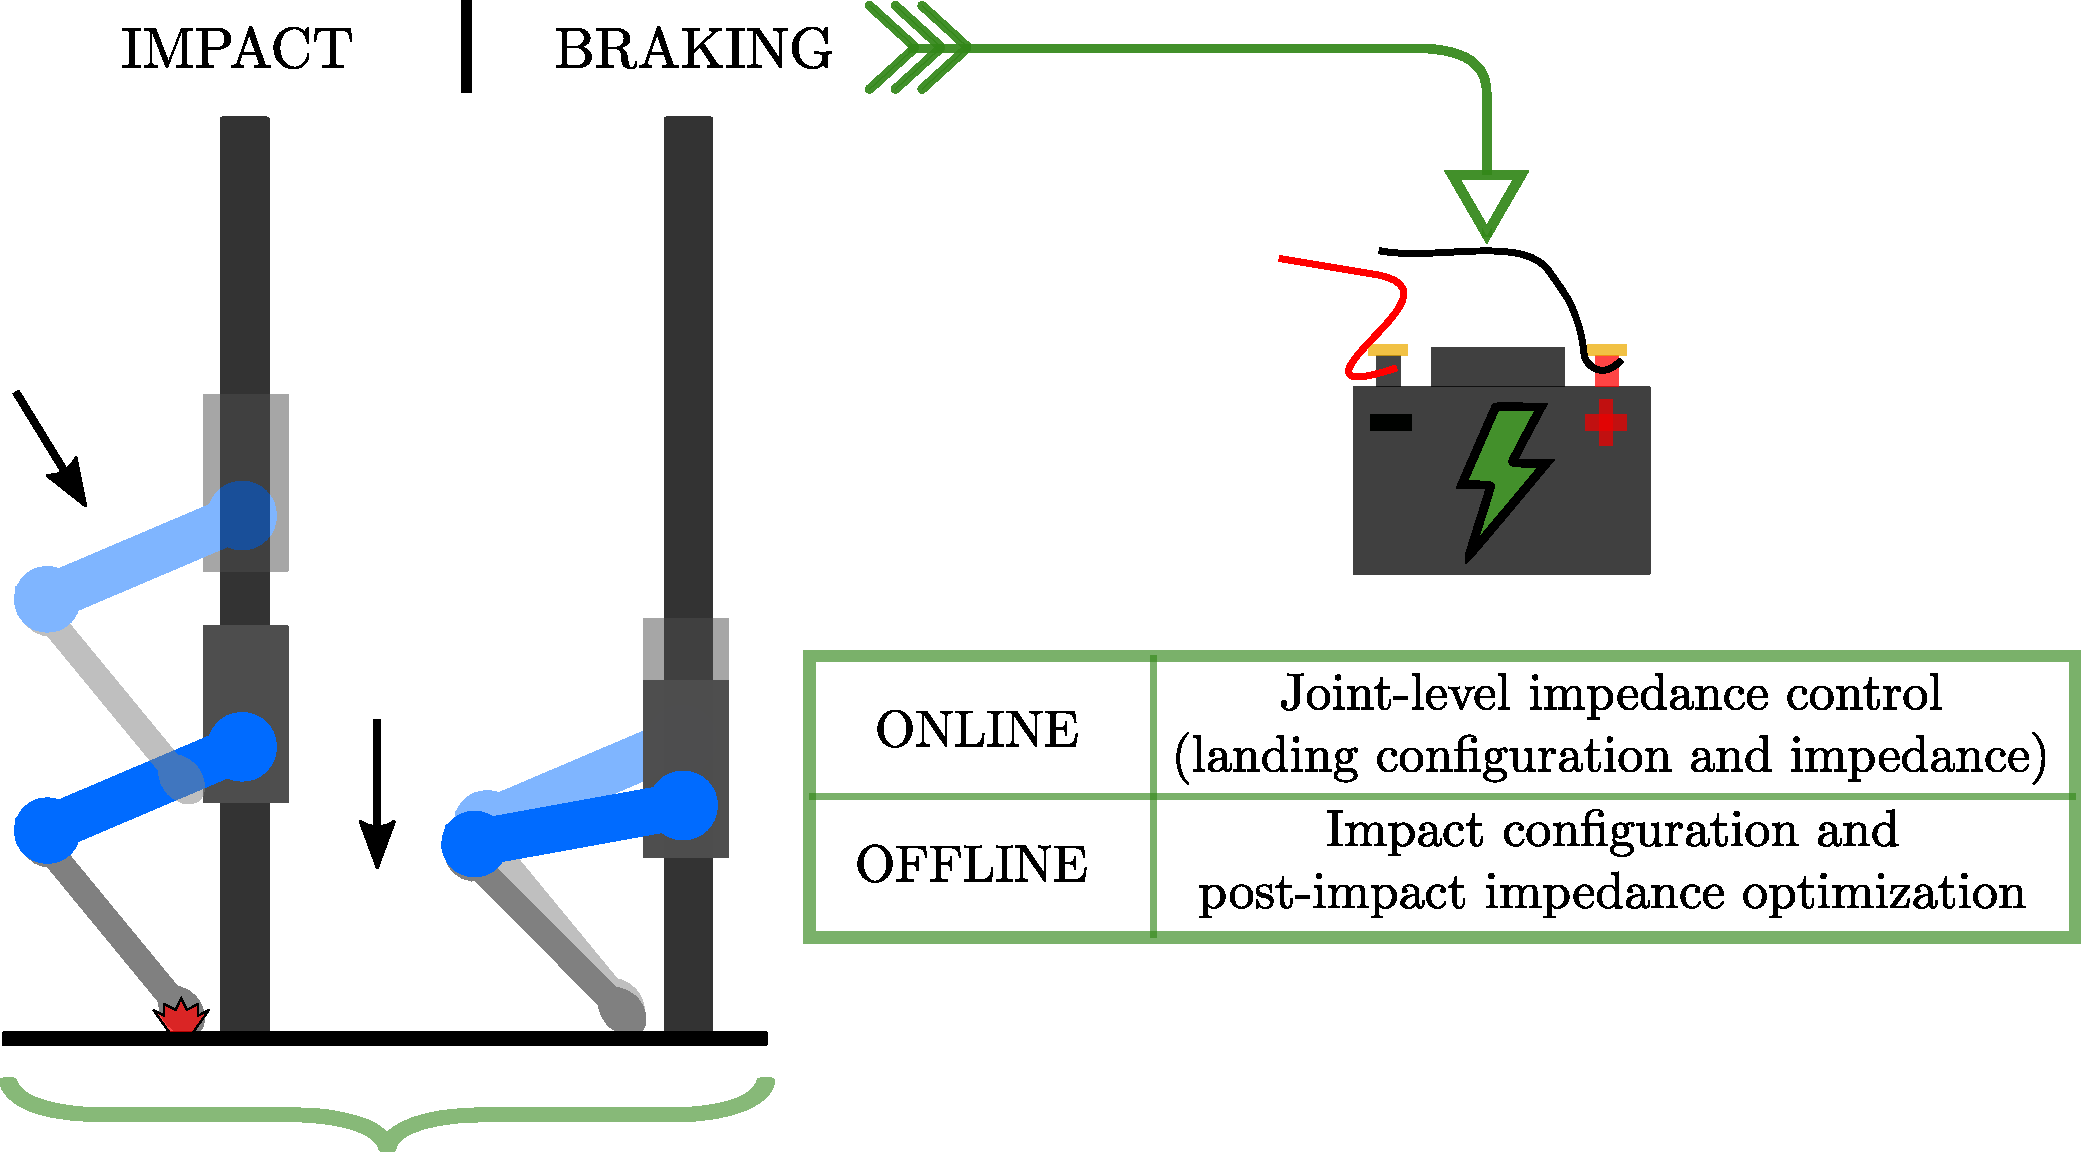
\includegraphics[width=1.0\columnwidth]{beamer_imgs/impact_opt_intro/second_TO.pdf}
\end{figure}
\end{multicols}
\end{frame}

%%%%%%%%%%%%%%%%%%%%%%%%%%%%%%%%%%%%%%%%%%%%%%%%%%%%%%%%%%%%%%%%%%
\begin{frame}
\begin{multicols}{2}
Jerk and yank regularization promotes \textbf{feasible} solutions $\rightarrow$
\vspace{0.3cm}
\begin{figure}
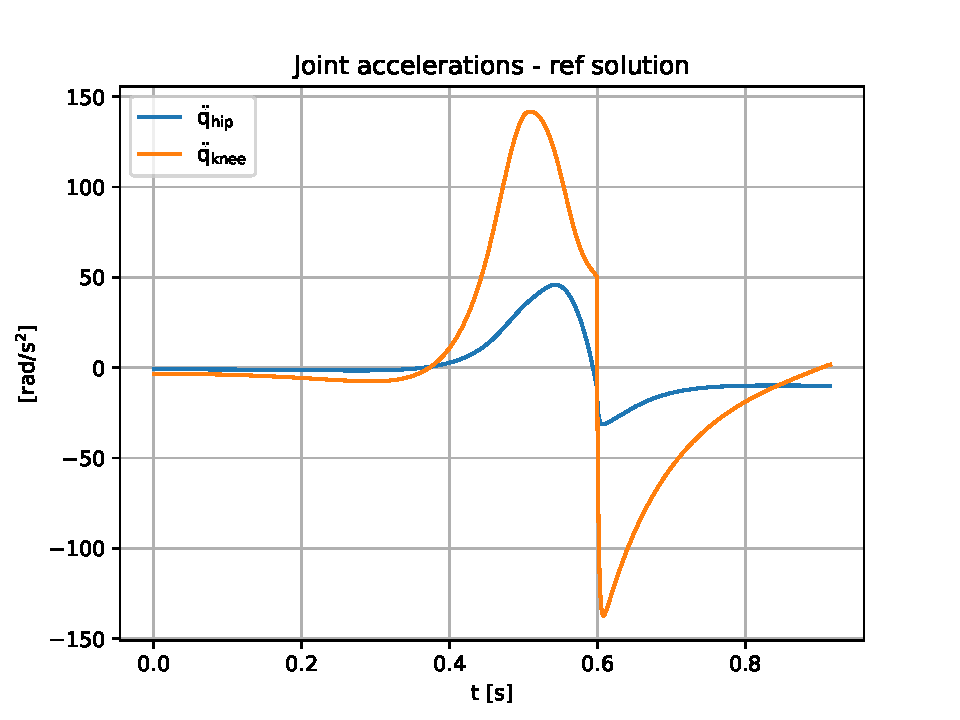
\includegraphics[width=1.0\columnwidth]{beamer_imgs/optimal_jumping_traj/ref/acc.pdf}
\end{figure}
\columnbreak
Resulting in \textbf{smooth}\\ TO inputs:
\begin{figure}
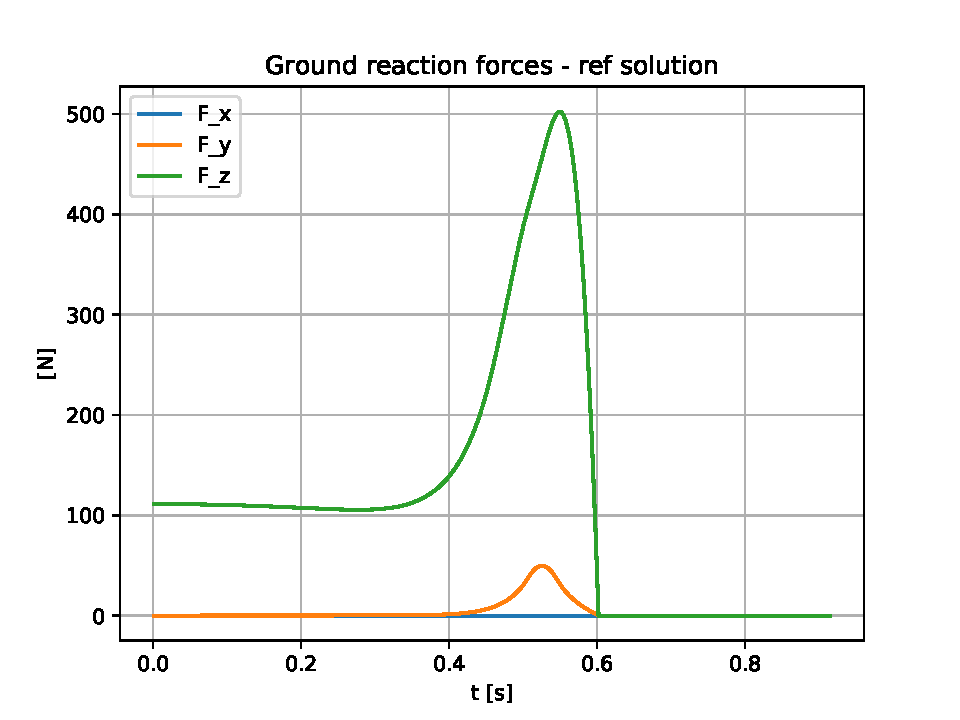
\includegraphics[width=1.0\columnwidth]{beamer_imgs/optimal_jumping_traj/ref/grf.pdf}
\end{figure}
\end{multicols}
\end{frame}

\begin{frame}
\begin{multicols}{2}
\vspace{0.5cm}\hphantom{e}\\
Optimal take-off trajectory \textbf{replay}:
\vfill\null
\columnbreak
\vspace{0.5cm}\hphantom{e}\\
Reduced optimization-to-reality gap:
\begin{figure}
    \centering
    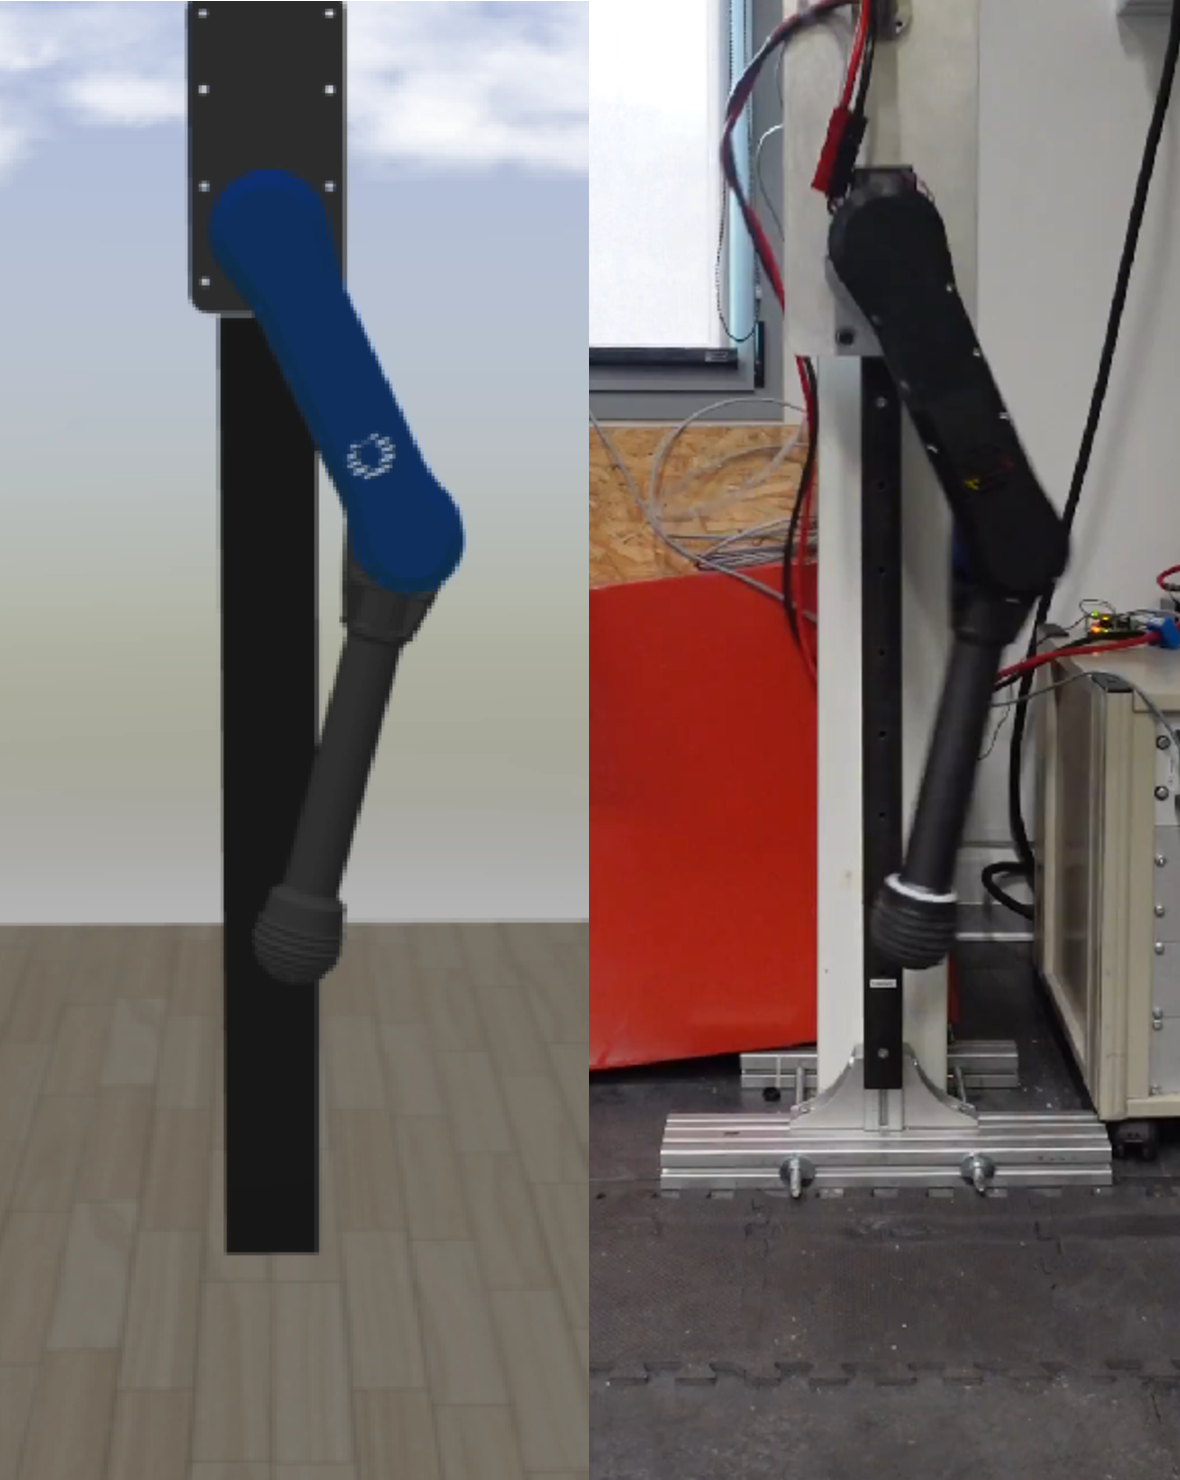
\includegraphics[width=0.5\columnwidth]{beamer_imgs/opt2sim.pdf}
\end{figure}
\end{multicols}
\end{frame}

%%%%%%%%%%%%%%%%%%%%%%%%%%%%%%%%%%%%%%%%%%%%%%%%%%%%%%%%%%%%%%%%%%

\begin{frame}
Measured regeneration @ touchdown:
\begin{itemize}
\item \textbf{optimal} take-off
\item \textbf{not}-\textbf{opt}. configuration/impedance
\item \textbf{real} robot
\end{itemize}
\begin{multicols}{2}
\begin{figure}
    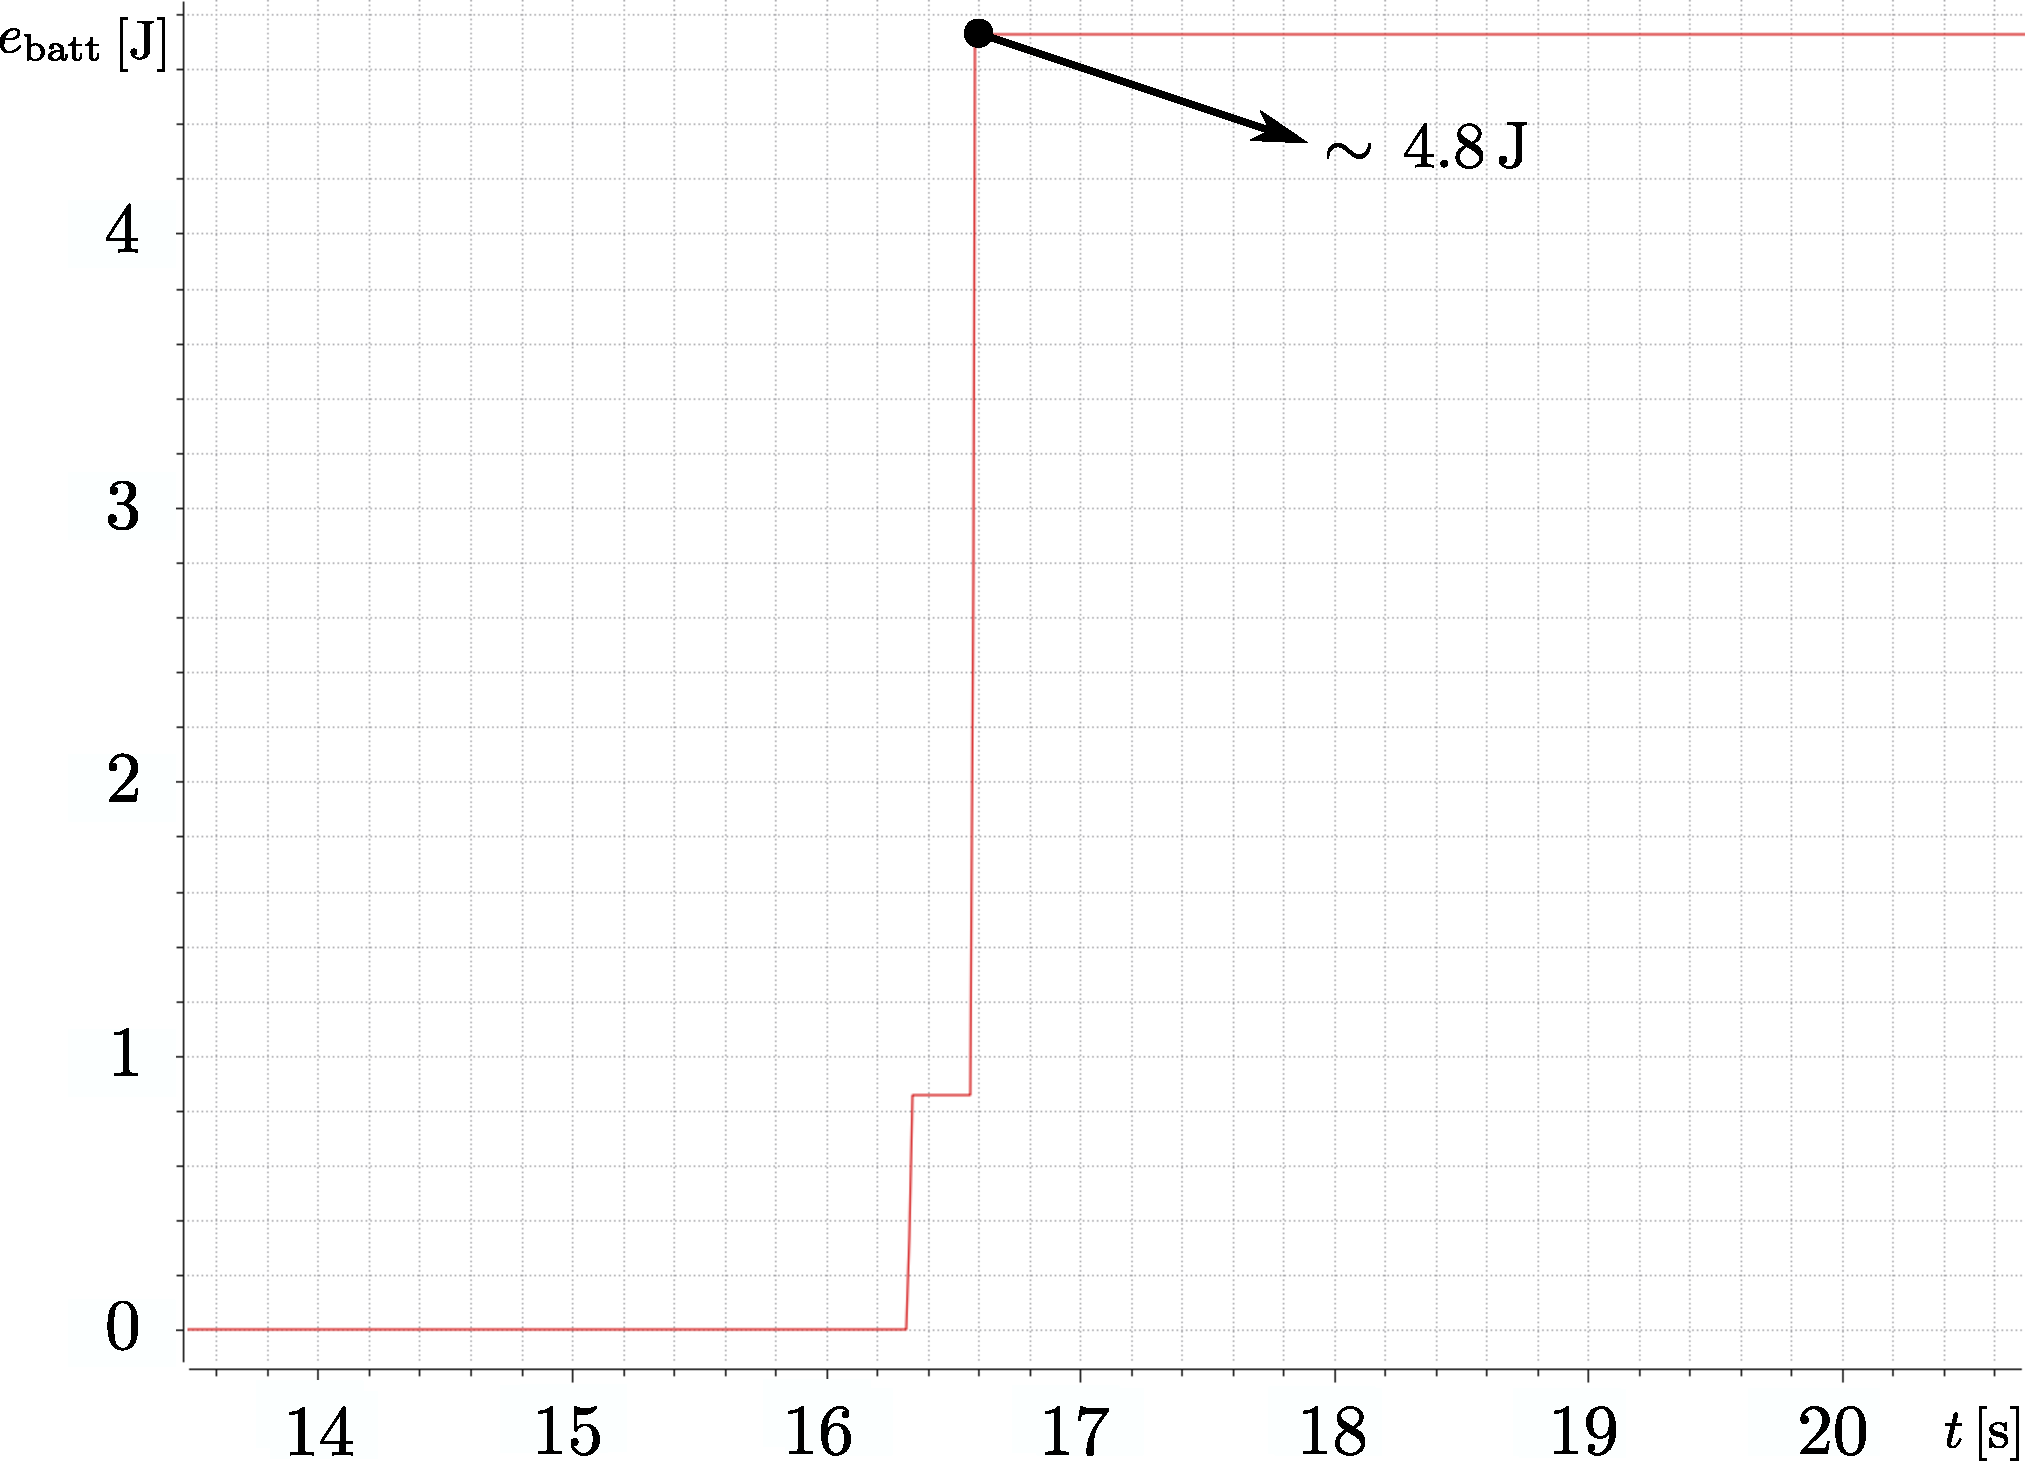
\includegraphics[width=1.0\columnwidth]{beamer_imgs/reg_energy.pdf}
\end{figure}
\columnbreak
\begin{figure}
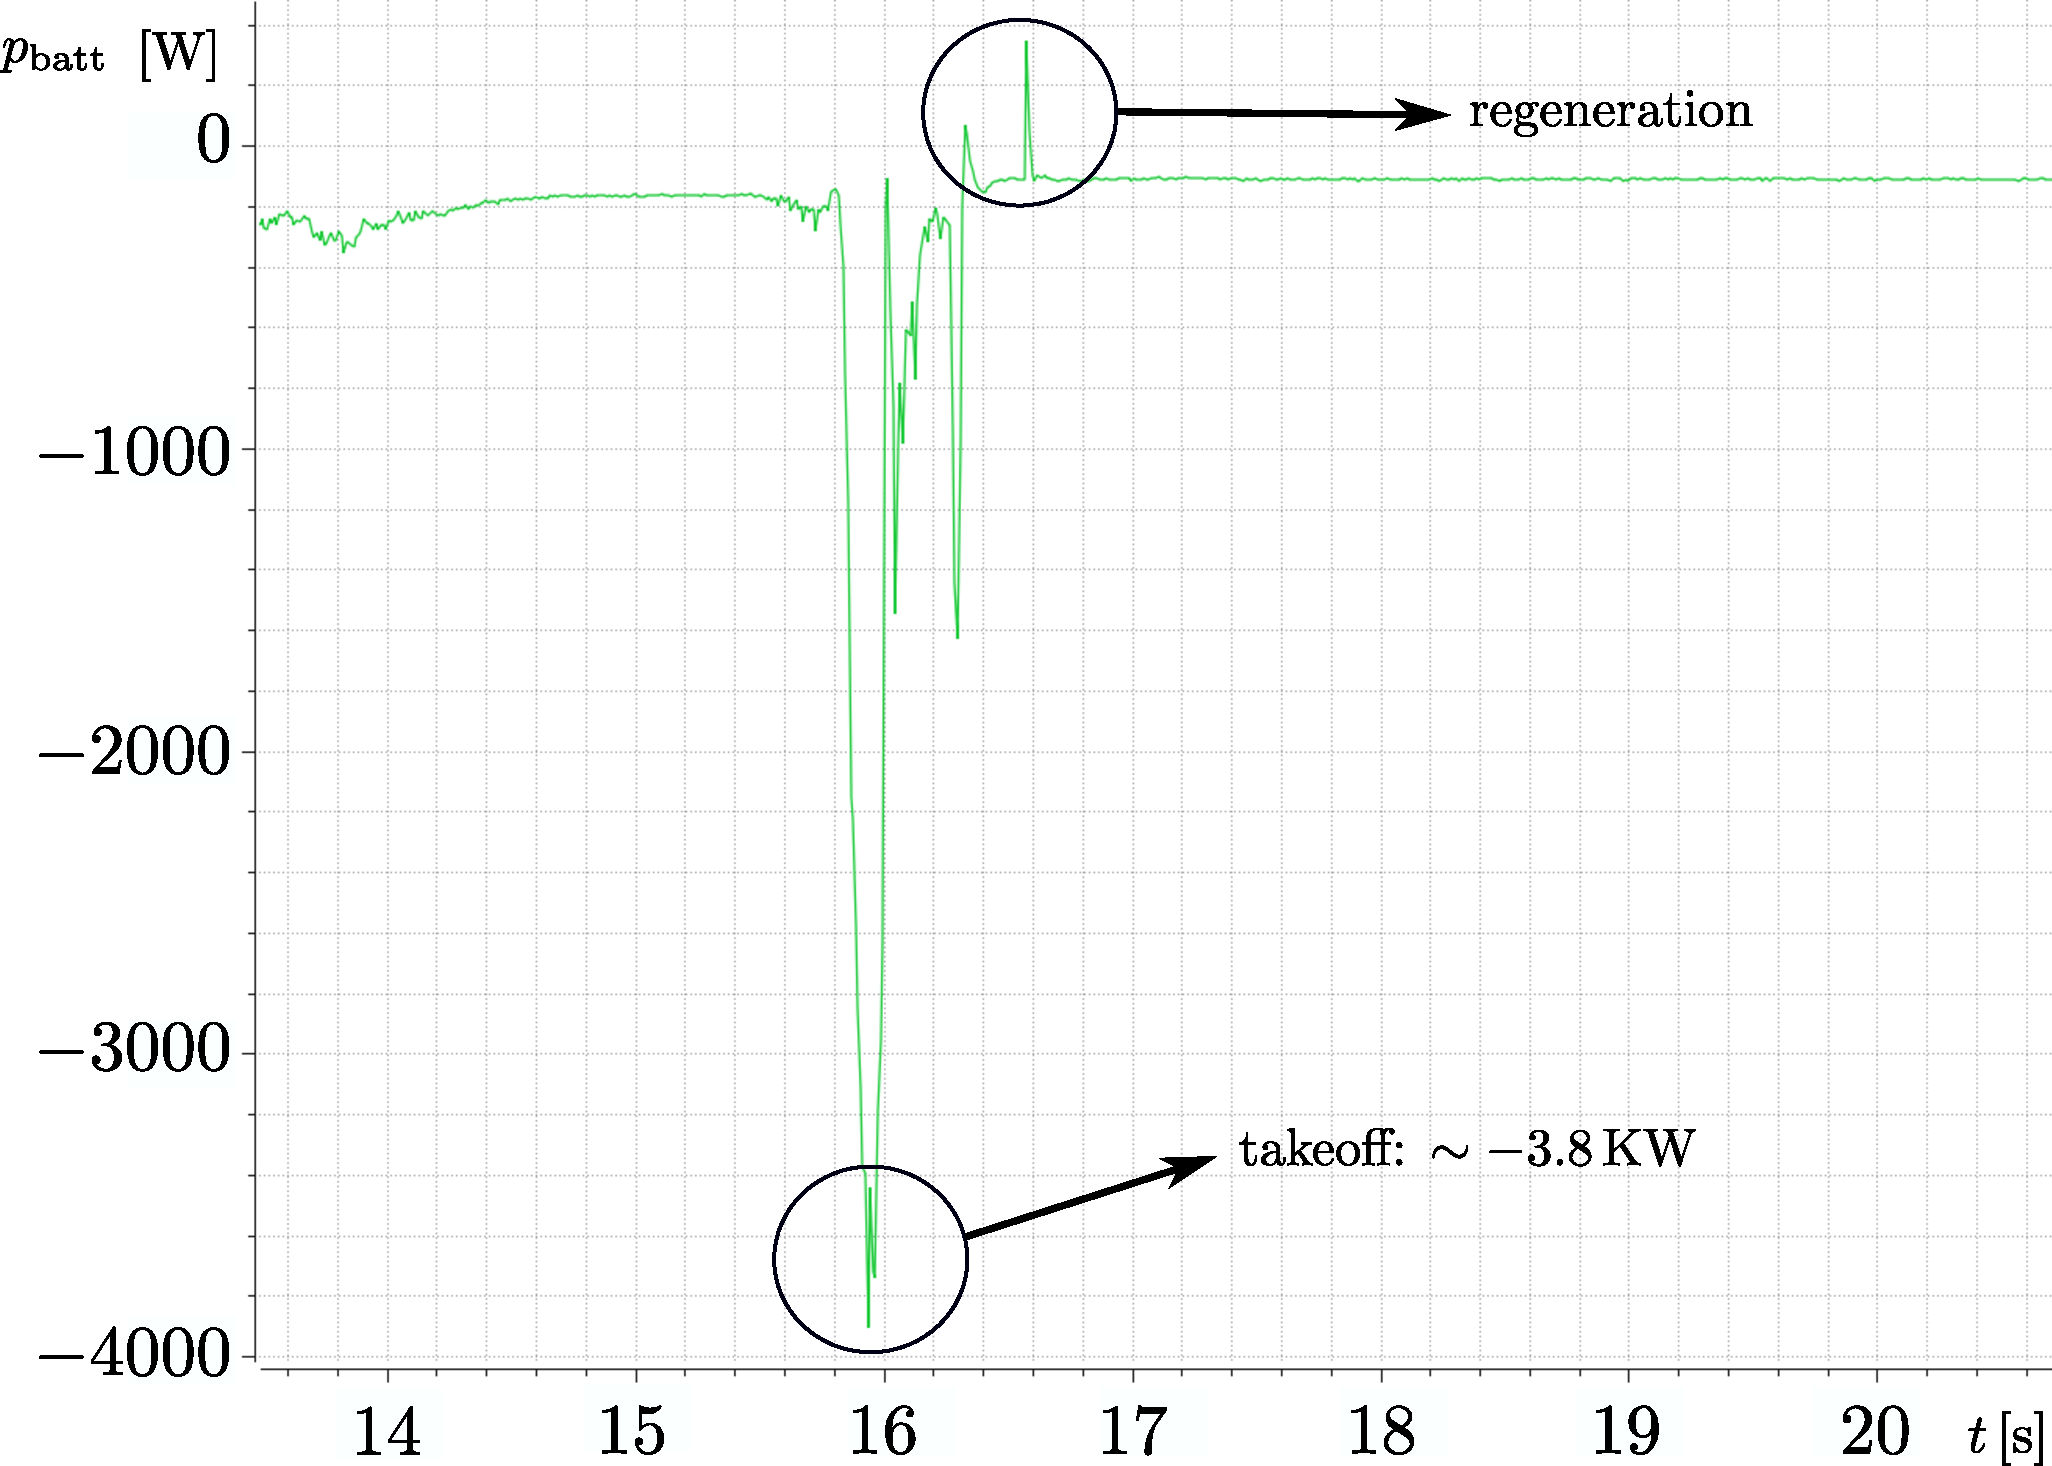
\includegraphics[width=1.0\columnwidth]{beamer_imgs/reg_pow.pdf}
\end{figure}
\end{multicols}
\end{frame}

%%%%%%%%%%%%%%%%%%%%%%%%%%%%%%%%%%%%%%%%%%%%%%%%%%%%%%%%%%%%%%%%%%


\begin{frame}
Estimated regeneration @ touchdown; successive jumping test:
\begin{itemize}
\item \textbf{optimal} take-off
\item \textbf{opt}. configuration/impedance
\item \textbf{simulated} robot
\end{itemize}
\begin{multicols}{2}
\begin{figure}
    \centering
    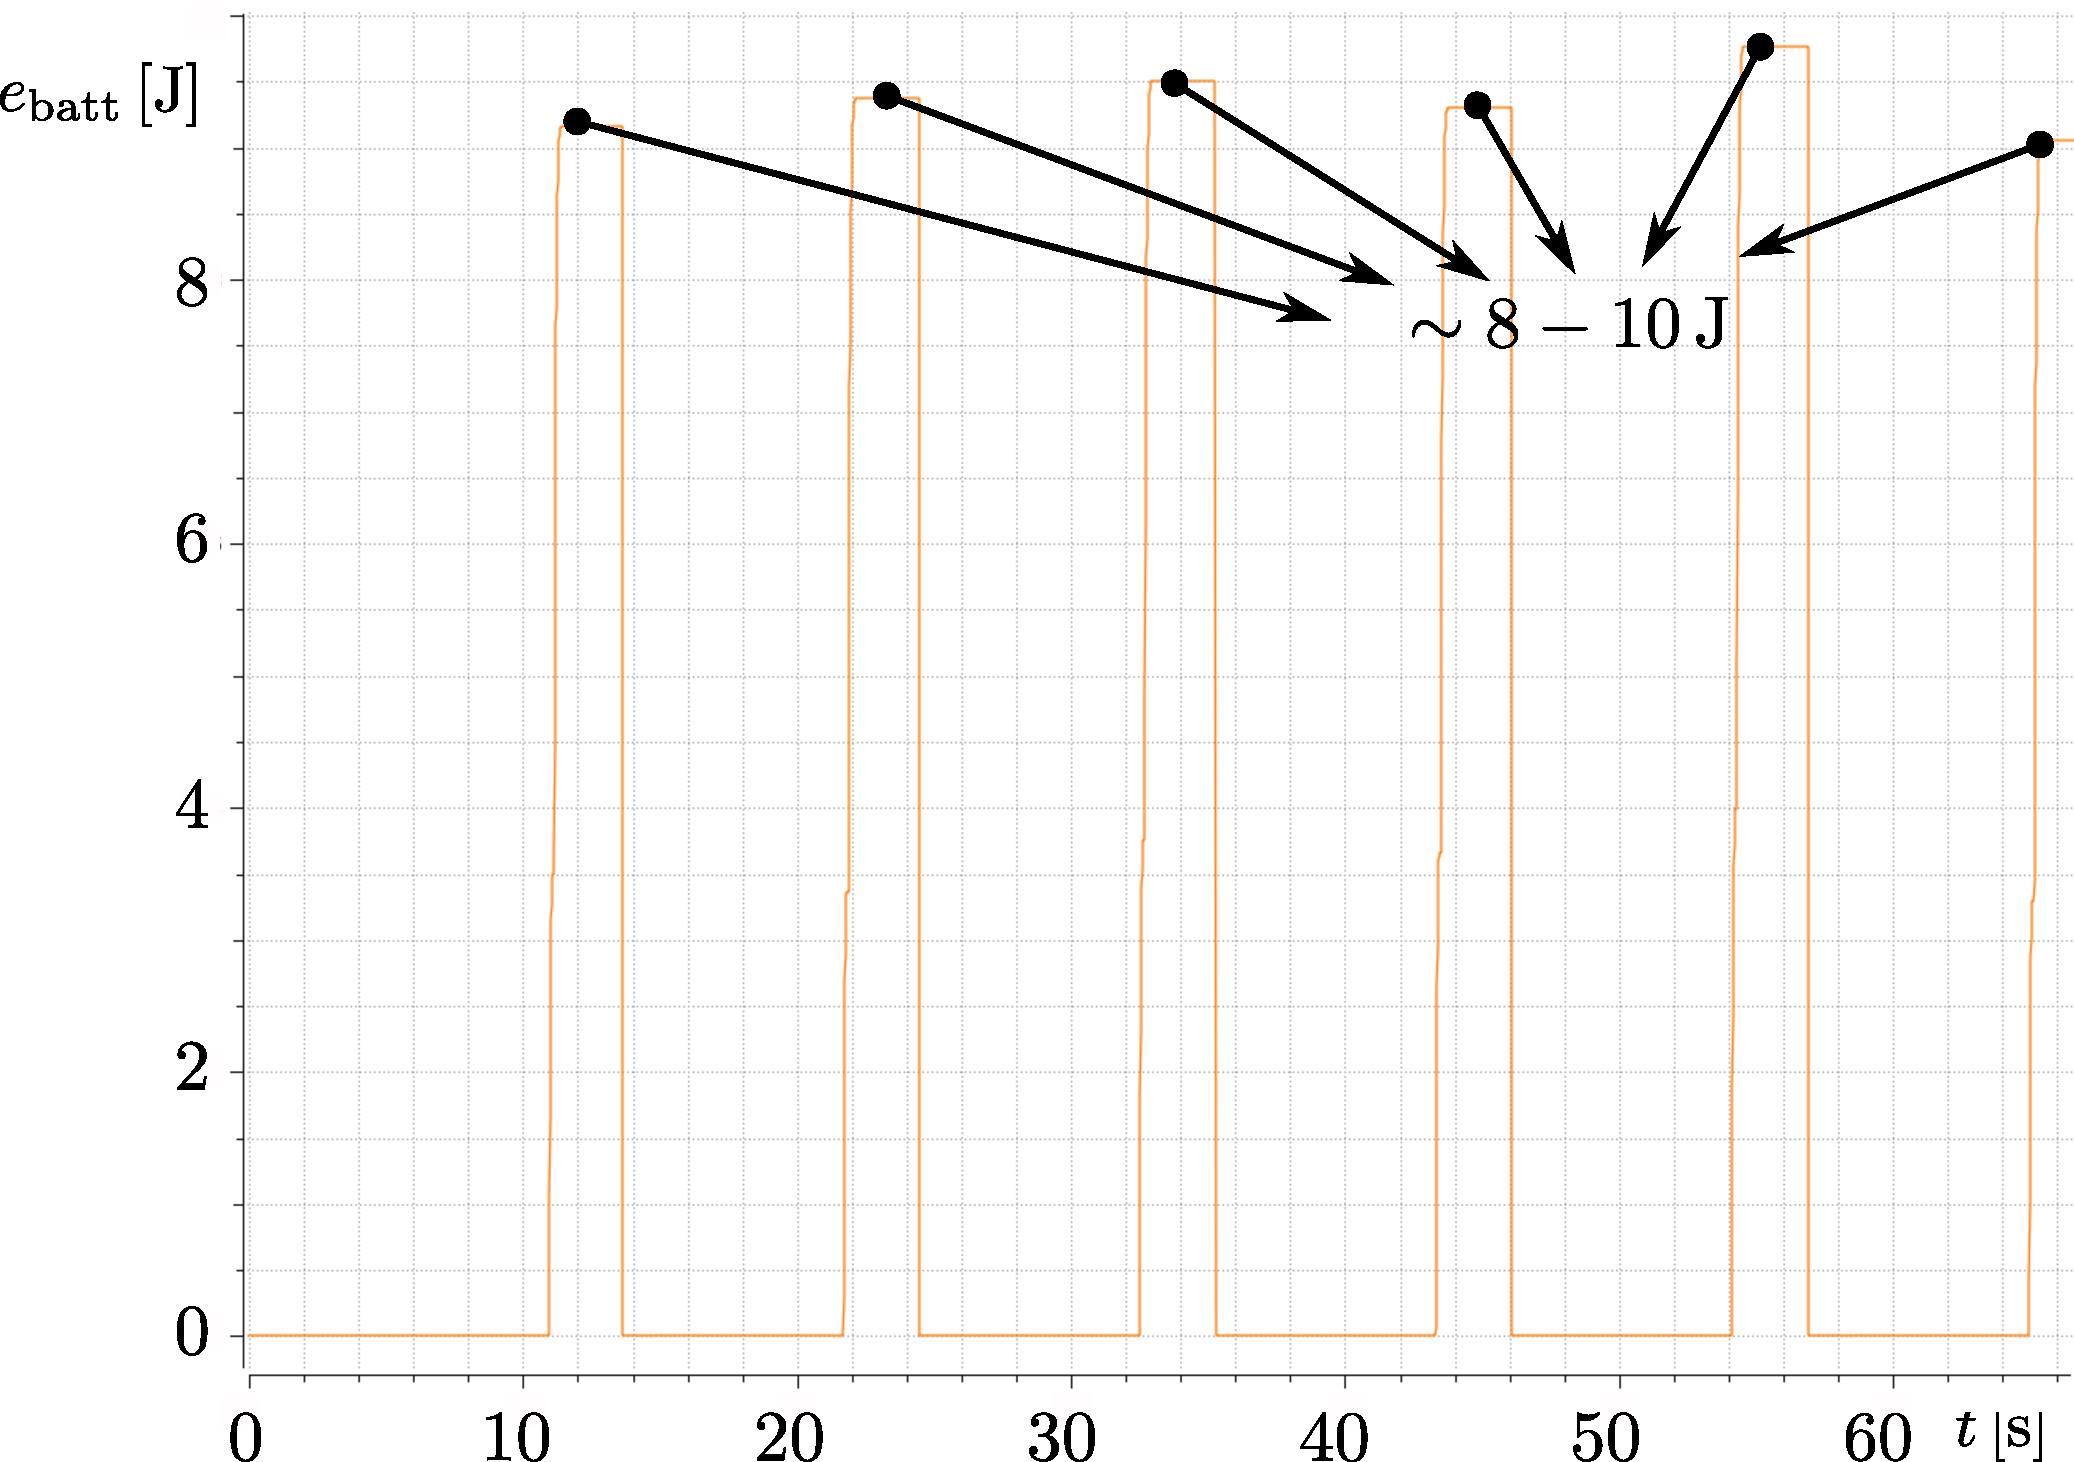
\includegraphics[width=1.0\columnwidth]{beamer_imgs/e_batt_sim.pdf}
\end{figure}
\vfill\null
\columnbreak
\centering
\begin{figure}
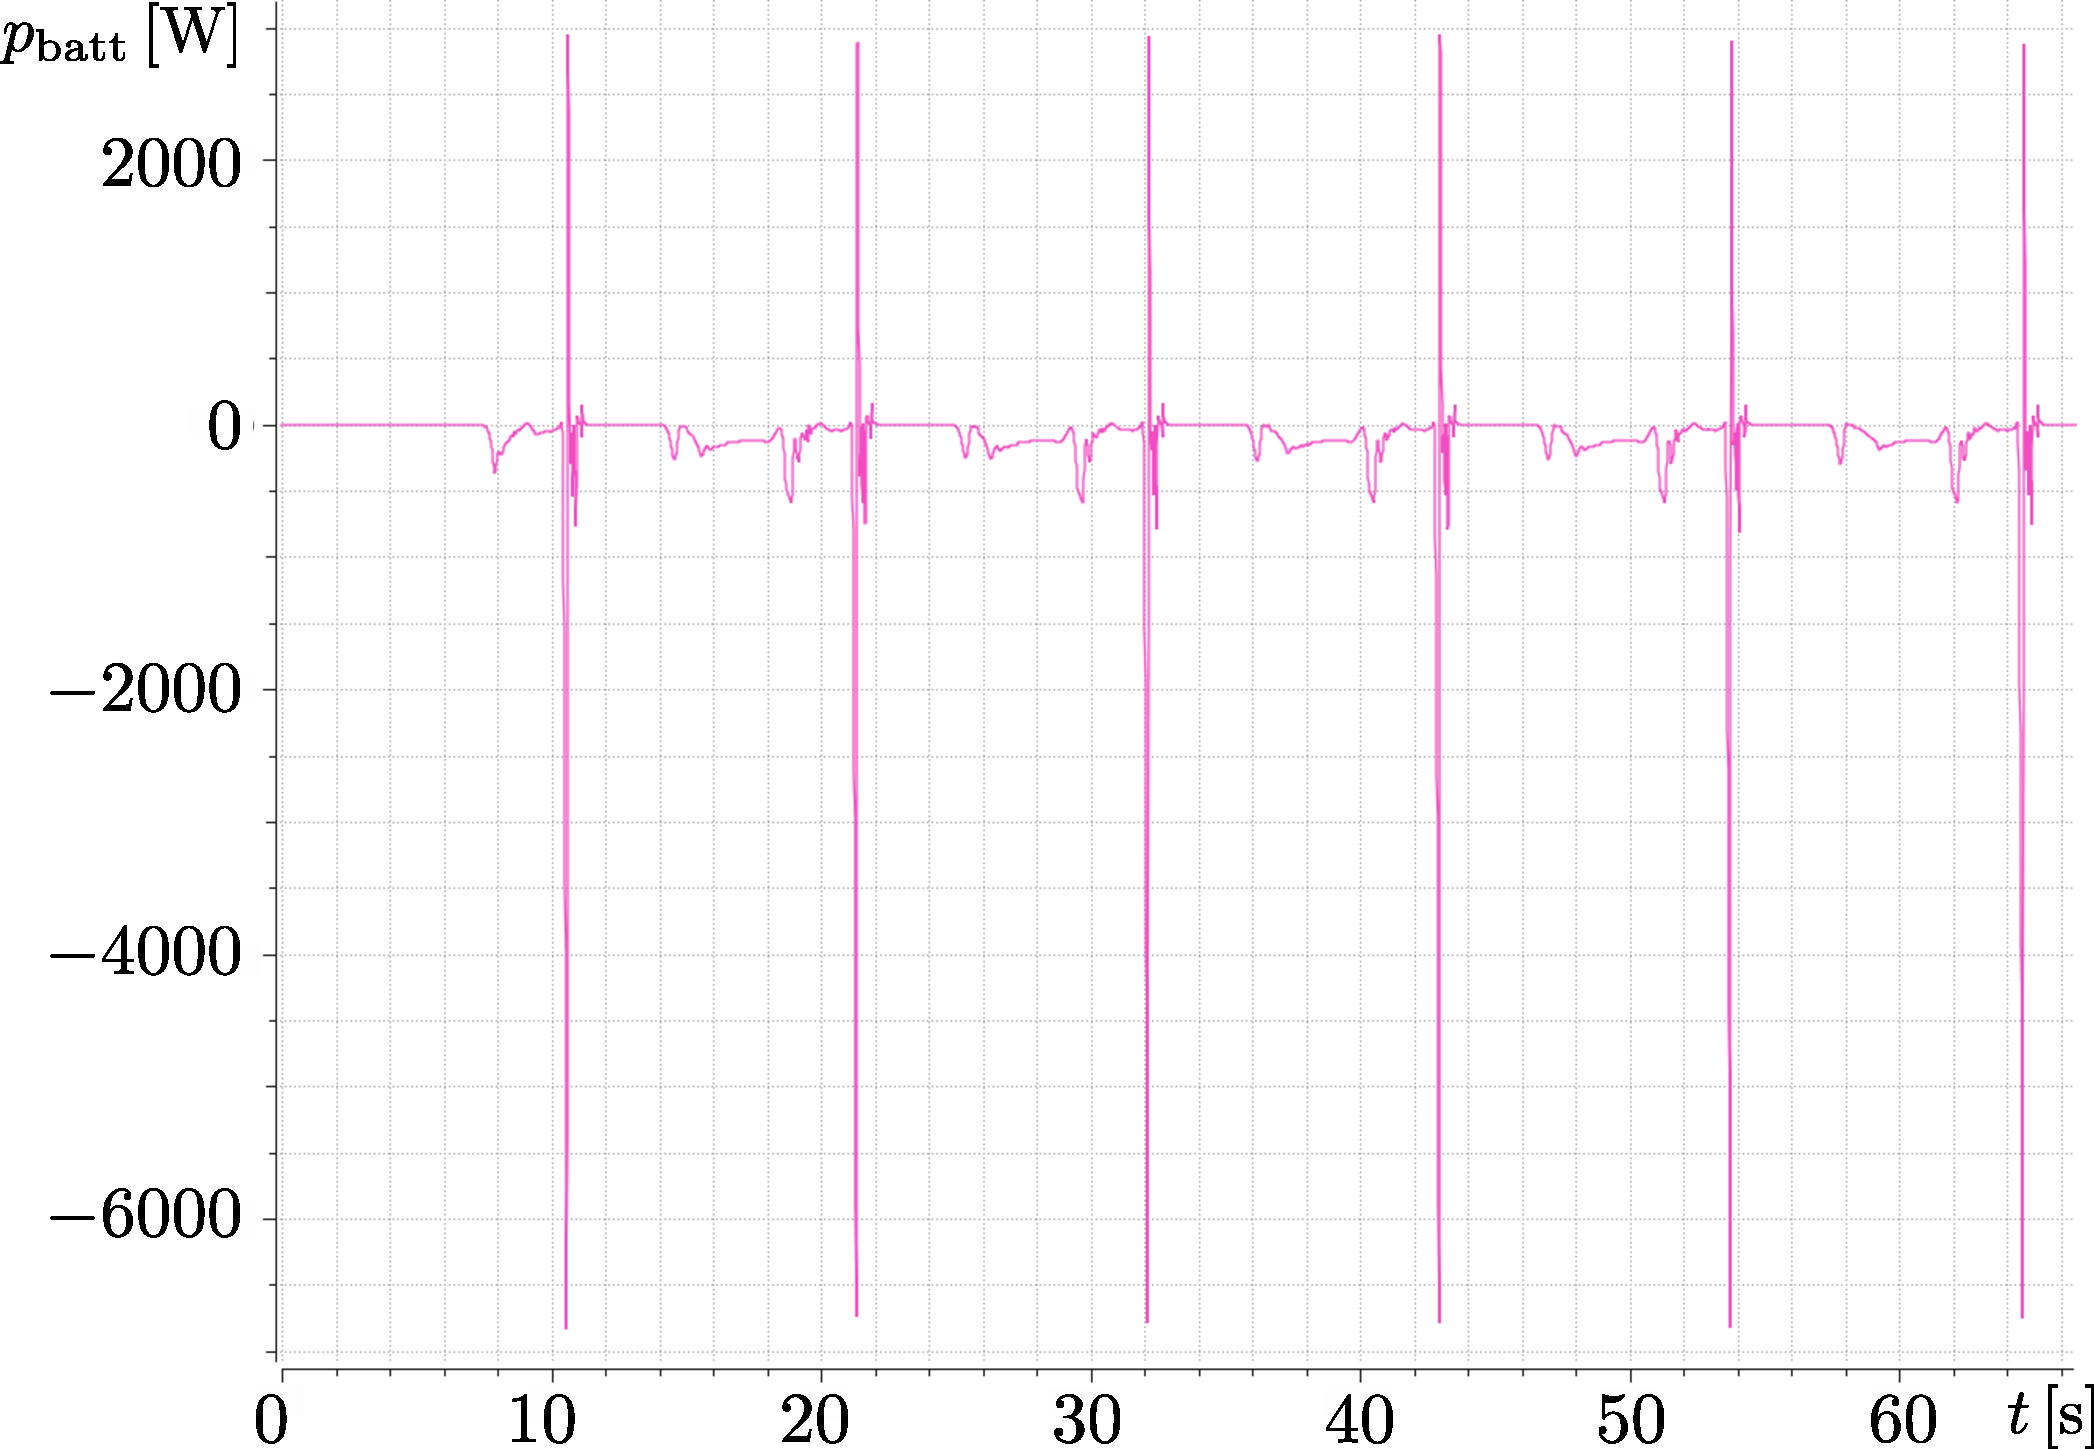
\includegraphics[width=1.0\columnwidth]{beamer_imgs/p_batt_sim.pdf}
\end{figure}
\vfill\null
\end{multicols}
\end{frame}


\titleframe



\end{document}
